\documentclass[journal, a4paper]{IEEEtran}


\usepackage{graphicx} 
\usepackage{url}      
\usepackage{amsmath}  \begin{document}
	\title{Algorithm and Optimization for Big Data}
	\author{Winter 2017\\ 
		\vspace{0.5cm}
		End Semester Examination\\
		\vspace{0.2cm}
		School of Engineering and Applied Sciences\\
		Ahmedabad University.
		\linebreak\linebreak
		Report by:\\ Neel Puniwala - 1401024}
		
	\maketitle
\begin{abstract}There are lots of amount of Candidate Profile is uploaded on the internet in professional world and these huge amount of data is received by the recruiter. Due to overload of unnecessary data recruiters task become very difficult. Job seeker also find difficult in seeking a job suitable for him or her. Recommendation system helps in this problem to make good choice. There are many algorithms such as Content based filtering, collaborative filtering on Data etc. I implemented content based filtering where candidate profile data is given and based on that module 1 and module 2 is working. I also have one other approach which is called graph based recommendation system.\\
	Index Terms \textendash Data cleaning, clustering, Text semantics, natural language, cosine factor, Content based filtering, recommendation system \textit{(key words)}
\end{abstract}


\section{Introduction}
	\PARstart{W}{hat} is recommendation systems? Why it is needed? These are the relevant questions and one need to answer these questions. Over a generating of huge amount of data, it is difficult to make nice choice or select the thing which is preferable for you. It is very time consuming and tedious job for people. This is where recommendation system came into existence. Basically recommendation system produce result which suitable for user choice and decreases the selection area. We can compare recommendation system with filter but there is one major difference between filters and recommendation system. In recommendation system filtering of data is done automatically where in filters user needs to apply manually on data. Recommendation systems mainly divides into two parts.     
	\begin{enumerate}
		\item Personalized Recommendation System
		\item Non-personalized Recommendation System
	\end{enumerate}
	
	Non-personalized system is the simplest recommendation system. This type of recommendation system does not focus on the user. Basically it will recommend the current trend to user and recommendation is not affect by user choice. One of the famous example of non-personalized example is YouTube Trending. It will show list of videos which are currently in trend when you first time login to You Tube. Now it is a case where you already login to You Tube and watch many video so next time when you open You Tube it will recommend video based on your previous search. This is what personalized recommendation system.  	
% Main Part
\section{MOTIVATION}
	As we saw recommendation system is very useful and we can reuse available data to recommend things to user. Idea is to use recommendation system in professional world. There is massive amount candidate profile data available we can use it to recommend career path. I have implemented two modules as a part of recommendation system for career path.
	\begin{enumerate}
		\item A module that read user profile and suggest a career path in term of skill set to be acquired
		\item A module in which user enter career goal and based on his career goal and other related information module will suggest a career path.
		
	\end{enumerate}
	
	In first module, candidate career profiles are available inn term of Data. Based on that data recommendation system is suggesting skills which to be acquired. But here challenge is to clean Data because Data can be available in different language, there are different type of Unicode used in the data. There are Job titles have multiple variations and same issue is faced in education degree. And content based recommendation system required huge amount of Data. To get useful data we need to first clean available data. In second module based on the career goal module will suggest skills which required for career goal. So these are the possible challenges to build content based recommendation system.   


\section{DATA CLEANING }
I implemented two ways to clean data. First way is to covert JSON file into CSV file. Converting helps to arrange given Data in column row format. Where first row is candidate ID, second row is for Additional Information and so on as we saw in Database. It is helpful to understand Data. In second way I used NLTK python package to clean data.
\begin{center}
	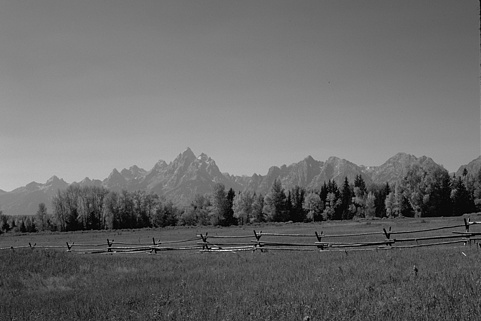
\includegraphics[width=8cm]{1}\\
\small	Fig.1 Cleaning data
\end{center}

\section{ALGORITHM}
As I discussed earlier I implemented recommendation system which use content based algorithm to give recommendation.	
\begin{center}
	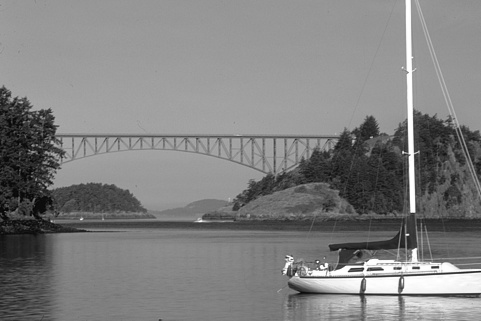
\includegraphics[width=8cm]{2}\\
	\small Fig.2 Content based filtering
\end{center}
After cleaning Data, I used data structure called dictionary in python (Similar to Hash map) to store all data profession wise. Where key is Name of the profession and its corresponding value is skills required for that profession. This makes my task easy for the creation of second module. Whenever user enter career goal algorithm will find key in dictionary and value of key given as Output. These skills are the union of the skills all present candidate have for particular profession. For first module same dictionary is useful. When candidate upload their profile to find skill similarity I used Pearson algorithm. It will find co-relation between uploaded profile and profile available in dictionary. Algorithm will give value between -1 to 1. 1 indicates skills are exactly matching and candidate is perfect for the Job and -1 indicates that both profiles are very different from each other.
\begin{enumerate}
	\item Find the skills that present in both profile
	\item If output of Pearson algorithm \textgreater 0.6 counter will increases
	\item Do step 1 and 2 for all the profile
	\item Maximum 3 value are profession which are suitable for uploaded profile
\end{enumerate}
Cosine similarity function is given as\\
$$simil(x,y) = cos(\overrightarrow{x},\overrightarrow{y})=\frac{\overrightarrow{x},\overrightarrow{y}}{\parallel \overrightarrow{x} \parallel_2 X \parallel \overrightarrow{y} \parallel_2}$$
$$ = \frac{\Sigma_{i \in l_{xy}} r_{x,i} r_{y,i}}{\sqrt{\Sigma_{i \in l_{xy}} r_{x,i}^2 \Sigma_{i\in l_{xy}} r_{y,i}^2}}$$

	\begin{center}
		
\includegraphics[width=8cm]{4}\\
		\small Fig.3 Flow of Program
	\end{center}


\section{Result}
	\begin{center}
		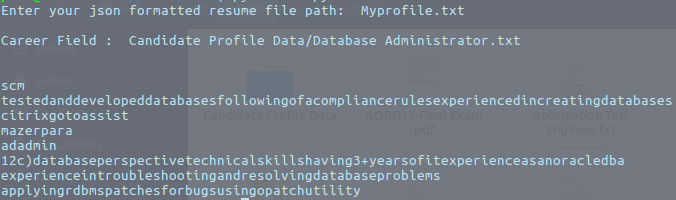
\includegraphics[width=8cm]{O1}\\
		\small Fig.4 Module 1 output
	\end{center}
	
	\begin{center}
		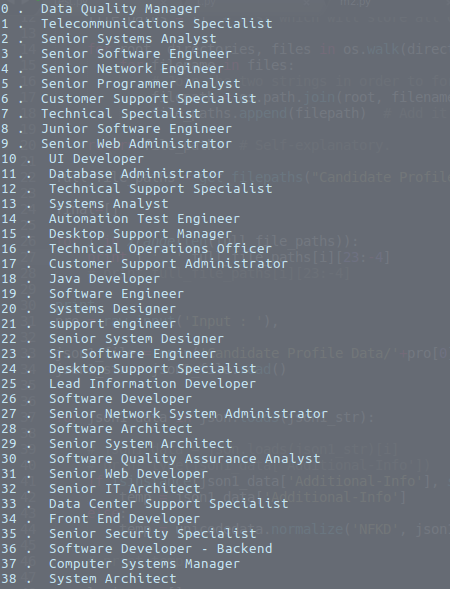
\includegraphics[width=8cm]{O21}\\
		\small Fig.5.1 Module 2 output 1
	\end{center}

	\begin{center}
			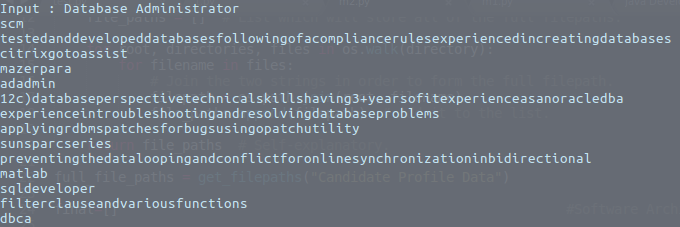
\includegraphics[width=8cm]{O22}\\
			\small Fig.5.2 Module 2 output 2
		\end{center}
\section{ANOTHER APPROACH}	
From given data we have list of candidate. We can make bipartite graph using common skills between candidate. Whenever new candidate come who connected to present user then algorithm can recommend common skills between two candidates. Depth of the path between candidate and skill is weight of the path.   

\begin{center}
	
\includegraphics[width=8cm]{3}\\
	\small Fig.6 Graph based recommendation system
\end{center}

\section{CONCLUSION}
Content based recommendation system will recommend skills and career path based on candidate profile and candidate career goal. Data cleaning is important part of recommendation system as unclean data can lead algorithm to wrong path and wrong recommendation will be generate by algorithm. Clustering of common skill set candidate is useful in making dictionary. Graph based recommendation system will cost high when depth of the graph is too much. But in terms of suggestions it performs better than content based filtering algorithm.
% Now we need a bibliography:
\begin{thebibliography}{9}
	\bibitem{1}
	Das,Shuvayan "Beginners Guide To Learn About Content Based Recommender Engine" Analytics Vidhya \url{https://www.analyticsvidhya.com/blog/2015/08/beginners-guide-learn-content-based-recommender-systems/}., 2017. Web. 
	\bibitem{2}
	"Introduction To Recommender Systems: A 4-Hour Lecture". Technocalifornia.blogspot.in. \url{http://technocalifornia.blogspot.in/2014/08/introduction-to-recommender-systems-4.html}, 2017. Web. 	
	\bibitem{3}
	"How To Calculate Cosine Similarity Given 2 Sentence Strings? Python". Stackoverflow.com. \url{http://stackoverflow.com/questions/15173225/how-to-calculate-cosine-similarity-given-2-sentence-strings-python}, 2017. Web. 
	\bibitem{4}
"Recommendation Systems: Principles, Methods And Evaluation". Sciencedirect.com.\url{http://www.sciencedirect.com/science/article/pii/S1110866515000341}., 2017. Web. 
\bibitem{5}
Xiang, "Recommender System Algorithm And Architecture", Slideshare.net \url{https://www.slideshare.net/xlvector/recommender-system-algorithm-and-architecture-13098396}, 2017. Web. 
\bibitem{6}
	"Recommendation System ", \url{http://infolab.stanford.edu/~ullman/mmds/ch9.pdf}, Web		
\end{thebibliography}

% Your document ends here!
\end{document}